\documentclass[a4paper, 12pt]{article} %type 

% Russian Language
\title{Отчет по лабораторной реботе по теме: "Численные методы решения уравнения переноса"}
\author{Латарцев Павел Б05-902б группа}
\date{2023}

\usepackage[left=1cm, top=2cm, right=1cm, bottom=2cm, nohead, nofoot]{geometry}
\usepackage[warn]{mathtext}
\usepackage[T2A]{fontenc}
\usepackage[utf8]{inputenc}
\usepackage[english, russian]{babel}
\usepackage{tikz}
\usepackage{lipsum}

\usepackage{amsmath,amssymb}
\usepackage{amsthm}

\usepackage{verbatim}

%\usepackage[demo]{graphicx}
\usepackage{caption}

\newcommand{\p}[1]{\mathbb{P}(#1)}
\newcommand{\E}{\mathbb{E}}
\newcommand{\D}{\mathbb{D}}

\begin{document}

\maketitle

\section{Условие} 
Шаблон № 6, начальное условие «полуэллипс», $\sigma = 0.25$

\begin{figure}[h!]
    \centering
    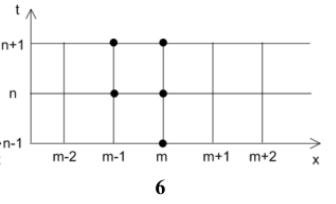
\includegraphics[width=10cm]{shablon.png}
    \caption{Схема шаблона}
    \label{fig:vac}
\end{figure} 

Начальное условие «полуэллипс»:
\begin{equation*}
\varphi(x) = 
 \begin{cases}
   \sqrt{1 - 100 \cdot \left( x - 0.5 \right)^2} &\text{при $0.4 \leqslant x \leqslant 0.6$}\\
   0 &\text{иначе}
 \end{cases}
\end{equation*}


\section{Теоритическая часть}
$$\alpha^{0}_{-1} - \text{ось x}, \,\,\,\, \alpha^{0}_{0} - \text{ось y}$$

\subsection{Система}
\begin{equation*}
\varphi(x) = 
 \begin{cases}
 	\alpha^{1}_{-1}\left(1 + \sigma \right) + \alpha^{0}_{-1} - \alpha^{-1}_{0} \sigma = \sigma  \\  
 	\alpha^{1}_{-1} + \alpha^{0}_{-1} + \alpha^{0}_{0} + \alpha^{-1}_{0}  = 1 \\
 	\alpha^{1}_{-1} \left( 1 + 2\sigma + \sigma^2 \right) + \alpha^{0}_{-1} + \alpha^{-1}_{0}\sigma^2 = \sigma^2 \\
 	\alpha^{1}_{-1} \left( 1 + 3\sigma + 3\sigma^2 + \sigma^3 \right) - \alpha^{0}_{-1} + \alpha^{-1}_{0}\sigma^3 = -\sigma^3 
 \end{cases}
\end{equation*}

\subsection{Область монотонности положительных по Фридрихсу $\alpha^\nu_\mu \geqslant 0$ схем}
\begin{equation*}
 \begin{cases}
 	\alpha^{0}_{-1} \geqslant 0  \\  
 	\alpha^{0}_{0} \geqslant 0 \\
 	\alpha^{-1}_{0} = \frac{1}{1+2\sigma} - \frac{\sigma}{1 + 2\sigma}\alpha^{0}_{-1} - \frac{1 + \sigma}{1 + 2\sigma}\alpha^{0}_{0} \geqslant 0 \\
 	\alpha^{1}_{-1} = \frac{2\sigma}{1+2\sigma} - \frac{1 + \sigma}{1 + 2\sigma}\alpha^{0}_{-1} - \frac{\sigma}{1 + 2\sigma}\alpha^{0}_{0} \geqslant 0 
 \end{cases}
\end{equation*}

\subsection{Однопараметрическое множество схем 2-го порядка аппроксимации}
$$\alpha^{0}_{-1} = \frac{-\sigma-1}{\sigma+1} \alpha^{0}_{0}+ \frac{2}{\sigma+1}$$

\subsection{Единственная схема 3-го порядка аппроксимации}
$$\alpha^{0}_{-1} = \frac{2\sigma}{\sigma + 1},\,\, 
  \alpha^{0}_{0} = \frac{2(\sigma - 1)}{\sigma + 1}, \,\,
  \alpha^{-1}_{0} = \frac{\sigma - 1}{2\sigma^2 + 3\sigma + 1},\,\,
  \alpha^{1}_{-1} = \frac{2\sigma(\sigma-1)}{(\sigma+1)(2\sigma + 1)}$$


\subsection{Схема 2-го порядка аппроксимации наиболее близкая к множеству положительных по Фридрихсу схем}

\subsection{Рисунок для заданного шаблона и числа Куранта}
\begin{figure}[h!]
    \centering
    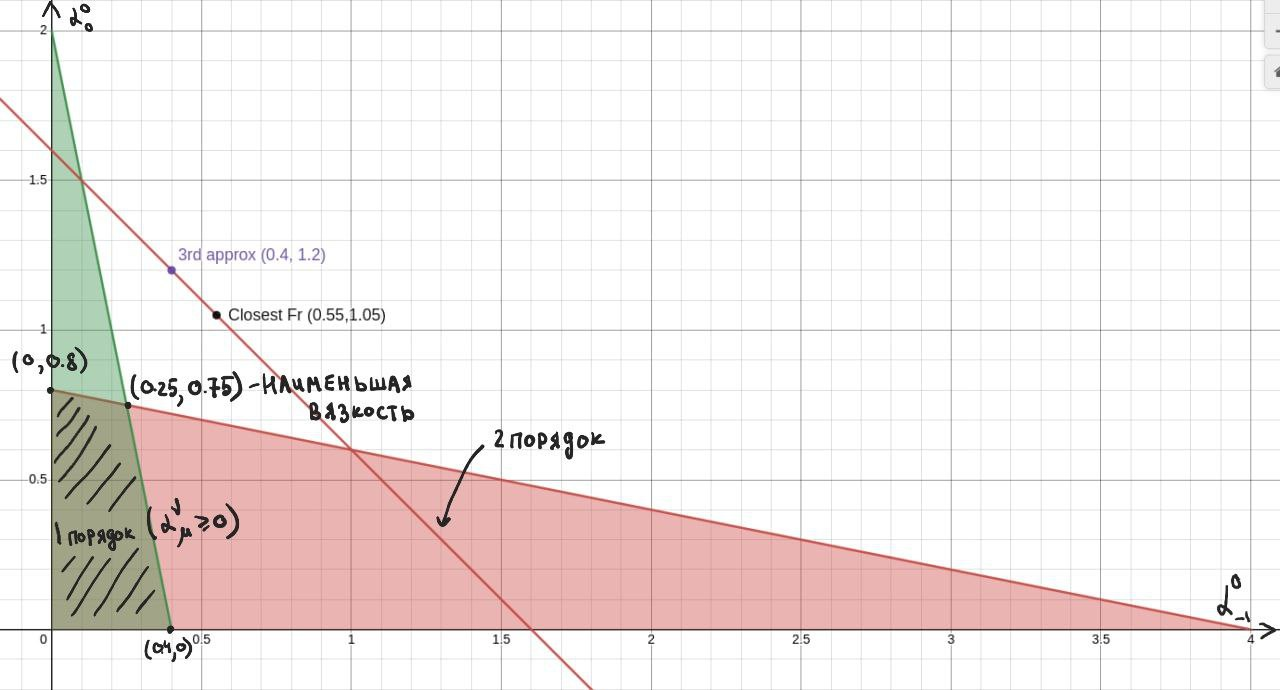
\includegraphics[width=17cm]{risunok.jpg}
    \caption{Рисунок для заданного шаблона и числа Куранта $\sigma = 0.25$}
    \label{fig:vac}
\end{figure} 


\section{Практическая часть}
\subsection{Четыре вершины области монотонных схем первого порядка аппроксимации}
\newpage
\begin{figure}[h!]
    \centering
    \includegraphics[width=15cm]{../graphs/First_order_approximation_right_up.png}
    \caption{Схема: $u^{n+1}_{m} = 0 \cdot u^{n+1}_{m-1} + 0.25 \cdot u^{n}_{m-1} + 0.75 \cdot u^{n}_{m} + 0 \cdot u^{n-1}_{m}$}
    \label{fig:vac}
\end{figure} 

\begin{figure}[h!]
    \centering
    \includegraphics[width=15cm]{../graphs/First_order_approximation_right_down.png}
    \caption{Схема: $u^{n+1}_{m} = 0 \cdot u^{n+1}_{m-1} + 0.4 \cdot u^{n}_{m-1} + 0 \cdot u^{n}_{m} + 0.6 \cdot u^{n-1}_{m}$}
    \label{fig:vac}
\end{figure} 

\begin{figure}[h!]
    \centering
    \includegraphics[width=15cm]{../graphs/First_order_approximation_left_up.png}
    \caption{Схема: $u^{n+1}_{m} = 0.2 \cdot u^{n+1}_{m-1} + 0 \cdot u^{n}_{m-1} + 0.8 \cdot u^{n}_{m} + 0 \cdot u^{n-1}_{m}$}
    \label{fig:vac}
\end{figure} 

\begin{figure}[h!]
    \centering
    \includegraphics[width=15cm]{../graphs/First_order_approximation_left_down.png}
    \caption{Схема: $u^{n+1}_{m} = \frac{1}{3} \cdot u^{n+1}_{m-1} + 0 \cdot u^{n}_{m-1} + 0 \cdot u^{n}_{m} + \frac{2}{3} \cdot u^{n-1}_{m}$}
    \label{fig:vac}
\end{figure} 

\newpage
\subsection{Наименее осциллирующая на разрывных решениях схема 2-го порядка аппроксимации из (5т) (Наиболее близкая ко множеству положительных по Фридрихсу схем)}
\begin{figure}[h!]
    \centering
    \includegraphics[width=15cm]{../graphs/Second_order_approximation_friedr_closest.png}
    \caption{Схема: $u^{n+1}_{m} = -0,3 \cdot u^{n+1}_{m-1} + 0.55 \cdot u^{n}_{m-1} + 1.05 \cdot u^{n}_{m} + -0.3 \cdot u^{n-1}_{m}$ \\ }
    \label{fig:vac}
\end{figure} 

\subsection{Две схемы 2-го порядка аппроксимации, лежащие на прямой – однопараметрическом множестве схем 2-го порядка аппроксимации – по разные стороны от схемы из (5т)}
\begin{figure}[h!]
    \centering
    \includegraphics[width=15cm]{../graphs/Second_order_approximation_1.png}
    \caption{Схема: $u^{n+1}_{m} = 0 \cdot u^{n+1}_{m-1} + 0.1 \cdot u^{n}_{m-1} + 1.5 \cdot u^{n}_{m} + -0.6 \cdot u^{n-1}_{m}$ \\ }
    \label{fig:vac}
\end{figure} 

\begin{figure}[h!]
    \centering
    \includegraphics[width=15cm]{../graphs/Second_order_approximation_2.png}
    \caption{Схема: $u^{n+1}_{m} = -0,6 \cdot u^{n+1}_{m-1} + 1 \cdot u^{n}_{m-1} + 0.6 \cdot u^{n}_{m} + 0 \cdot u^{n-1}_{m}$ \\ }
    \label{fig:vac}
\end{figure} 

\newpage
\subsection{Схема 3-го порядка аппроксимации}
\begin{figure}[h!]
    \centering
    \includegraphics[width=15cm]{../graphs/Third_order_approximation.png}
    \caption{Схема: $u^{n+1}_{m} = -0,2 \cdot u^{n+1}_{m-1} + 0.4 \cdot u^{n}_{m-1} + 1.2 \cdot u^{n}_{m} + -0.4 \cdot u^{n-1}_{m}$ \\ }
    \label{fig:vac}
\end{figure}







\end{document}




\begin{figure}[h!]
    \centering
    \includegraphics[width=20cm]{pr2.png}
    \caption{Функия распределения $\xi, \eta$.}
    \label{fig:vac}
\end{figure} 